\documentclass{article}
\usepackage[utf8]{inputenc}




\documentclass[12pt,a4paper]

\usepackage[utf8]{inputenc}
\usepackage[T1]{fontenc}
\usepackage{amsmath}
\usepackage{makeidx}
\usepackage{graphicx}
\usepackage{float}
\usepackage[width=17.00cm, height=24.00cm]{geometry}
\usepackage[polish]{babel}

\usepackage{hyperref}
\usepackage{listings}
\usepackage{color}

\newcommand{\AASprTab}[5]{


\begin{center}
\begin{tabular}{ p{0.06\textwidth} p{0.2\textwidth} p{0.2\textwidth} p{0.2\textwidth} p{0.2\textwidth} p{0.2\textwidth} }

  &   &   &   &   \\
\hline
%Tytuł dokumentu
\multicolumn{6}{|c|}{}\\[-1ex]
\multicolumn{6}{|c|}{{\LARGE Optymalizacja niewielkiego gospodarstwa rolnego}} \\
\multicolumn{6}{|c|}{}\\[-1ex]



\hline
\multicolumn{2}{|l|}{\AASprTabFieldDsc{Wydział}} & \multicolumn{2}{|l|}{\AASprTabFieldDsc{Kierunek}} & \multicolumn{2}{|l|}{\AASprTabFieldDsc{Rok}} \\
\multicolumn{2}{|c|}{\AASprTabFieldVar{EAIiIB}} & \multicolumn{2}{|c|}{\AASprTabFieldVar{Automatyka i Robotyka}} & \multicolumn{2}{|c|}{\AASprTabFieldVar{III}} \\



\hline
\multicolumn{1}{|c|}{\tiny{ }} &
\multicolumn{5}{|c|}{\tiny{ }} \\
\multicolumn{1}{|c|}{\AASprTabFieldDscH{L.p.}} &
\multicolumn{5}{|l|}{\AASprTabFieldDscH{Skład grupy ćwiczeniowej}}\\

\hline
\multicolumn{1}{|c|}{1} &
\multicolumn{5}{|l|}{\AASprTabFieldVar{#3}}\\

\hline
\multicolumn{1}{|c|}{2} &
\multicolumn{5}{|l|}{\AASprTabFieldVar{#4}}\\

\hline
\multicolumn{1}{|c|}{3} &
\multicolumn{5}{|l|}{\AASprTabFieldVar{#5}}\\

\hline
\end{tabular}
\end{center}
}

\renewcommand\lstlistingname{Quelltext}

\lstset{ % General setup for the package
	language=Python,
	basicstyle=\small\sffamily,
	numbers=left,
	numberstyle=\tiny,
	frame=tb,
	tabsize=4,
	columns=fixed,
	showstringspaces=false,
	showtabs=false,
	keepspaces,
	commentstyle=\color{red},
	keywordstyle=\color{blue}
}




\begin{document}

\AASprTab { Asynchroniczny silnik klatkowy z falownikiem }{16 grudnia 2022 r.}{Bartłomiej Matuszewski}{Piotr Mamos}{Dawid Maziarski}

\tableofcontents

\section{Wstęp}
Celem projektu była optymalizacja jednego z wymyślonych przez nasz problemów za pomocą poznanych na zajęciach algorytmów oraz innych źródeł (doradzanych przez prowadzącego).
Poniżej przedstawiamy rozwazane przez nas pomysły:
\begin{itemize}
	\item Pomysł zaproponowany przez Dawida zakładał optymalizacje wydatków związanych z zakupem opału w sezonie grzewczym z uwzględnieniem najważniejszych zależności fizycznych mających wpływ na temperature panujących w typowym domu jednorodzinnym.
	\item Pomysł Piotra skupiał się na planowaniu upraw dla niewielkiego gospodarstwa rolnego z uwzględnieniem uproszczonego modelu jakości ziemi oraz wpływu upraw na jakość gleby, w taki sposób by ostateczny zysk był jak największy. .
	\item Pomysł Bartłomieja bazował na maksymalizacji jakości komponentów w składanym komputerze przy jednoczesnej minimalizacji poniesionych kosztów
\end{itemize}

Wspólnie podjeliśmy decyzję iż z uwagi na największą elastyczność w kontekście złożoności zagadnienia, najbardziej rozsądną dla nas opcją będzie pomysł Piotra.

Następnie w ramach naszych zajeć wybrany problem przełożyliśmy na model matematyczny oraz zaimplementowaliśmy program który go optymalizuje.

\section{Model matematyczny}

	\subsection{Skrócony opis problemu:}
	Problem polega na stworzeniu kilkuletniego planu upraw dla niewielkiego gospodarstwa rolnego w zależności od zmiennej kategorii jakości gleby (w postaci cyfry w zakresie od 0 - 100) i  odległości uprawy od gospodarstwa. Celem będzie maksymalizacja zysków . Zakładamy przy tym że co roku nabywamy nowy materiał siewny.

	\subsubsection{Stałe:}
	\begin{itemize}
		\item N - Liczba dostępnych pól uprawnych.

		\item Y - liczba lat planowania upraw.

		\item T - stały koszt dojazdu na kilometr

		\item P - powierzchnia pola uprawnego w hektarach (każde pole ma identyczną powierzchnię)

		\item $ D_i $ -  Odległość i-tego pola od gospodarstwa, gdzie i = 1,...,N

		\item $ C_x $ - koszt produkcji danej rośliny na jeden hektar (koszt materiału siewnego, koszt pracy ludzkiej, itp.), gdzie x - nazwa rośliny

		\item $ W_x $- wpływ uprawy na glebę (zależne od uprawianej rośliny)

		\item $ S_x $ - zsumowana ilość dopłat i  wszelkich dodatków (w zależności od uprawianej rośliny)

		\item $ G = [g_{qx}] $ - macierz zysków z pola gdzie komórka  $ g_{qx} $ zawiera zysk z danej rośliny w zależnie od jakości gleby q i uprawianej rośliny $ x $.
	\end{itemize}

	\subsubsection{Zmienne:}
	\begin{itemize}
		\item $y$ - Obecny rok, y = 1,...,Y

		\item $ Q = [ q_{yi} ]_{Y \times N} $ -  Macierz klas jakości gleby gdzie komórka $ q_{yi} $ zawiera jakość ziemi którą na i-tym polu w roku y.
	\end{itemize}

	\subsubsection{Postać rozwiązania:}
	\begin{itemize}
		\item $ X = [x_{yi}]_{Y \times N} $ - macierz decyzyjna o wymiarach $ Y \times N $, gdzie komórka $ x_{yi} $ zawiera indeks rośliny którą siejemy na i-tym polu w roku y.
	\end{itemize}

	\subsubsection{Postać funkcji celu:}
	\begin{flalign}
		f(X) = \sum_{y=1}^{Y} \sum_{i=1}^{N} G_{q_{yi} x_{yi}} + S_{x_{yi}} - (C_{x_{yi}} * P + D_i * T)
		\\q_{yi} = q_{(y-1)i} + W_{x_{(y-1)i}}
	\end{flalign}

	\subsubsection{Ograniczenia:}
	\begin{itemize}
		\item $ 0 \leq q_{yi} \leq 100 $ Jakość gleby może zmieniać się w zakresie od 0 do 100
		\item $ x_{i-1} \neq x_i $, gdzie $ x_k $ nie jest stanem pustym pola
	\end{itemize}


\section{Implementacja}
Do realizacji naszego problemu wybraliśmy jezyk Python z bibiotekami QtGui, numpy, random oraz math z którego korzystaliśmy przede wszytskim z pomocą środowiska programistycznego Pycharm firmy JetBrains,
wybór ten był spowodowany wewnetrzną konsulatcją w grupie znajomości i upodobań co do poszczególnych języków i środowisk.
Przed przystąpieniem do fazy implementacji potrzebowaliśmy jeszcze znaleźć dane związane z kosztem dojazdu do pola za każdy kilometr oraz kosztów i przychodów związanych z każdą z upraw. Informację te znaleźlśmy w internecie, w szczególności, wiele danych bazowaliśmy na stornach wielkopolskiej izby rolniczej oraz mazowieckeigo ośrodka doradztwa rolniczego.
Niestety nie byliśmy wstanie znaleźć informacji co do plenności upraw na danej glebie oraz dokładnego wpływu każdej z upraw na glebe, dlatego zależności te zostały ustalone zgodnie z naszą wiedzą i obserwacjami oraz zdawkowymi informacjami znalezionymi w internecie, dużym uproszczenie jest jednak przyjęcie przez nas założenia iż każda z roślin ma identyczny (w każdym jednak przypadku odpowiednio przeskalowany) wykres zysku od jakości gleby.
Założyliśmy również zgodnie panującymi zaleceniami dotyczącymi znamionnowści upraw iż dana roślina nie będzie uprawia na danym polu dwa lata z rzędu (co również jest uproszczeniem w stosunku do rzeczywistości), jedym wyjątkiem było zostawienie ugoru na polu.
Zgodnie z rzeczywistością zaniechaliśmy jednak stosowania funkcji kary w stosunku do jakości gleby i ustaliliśmy iż jakość  ta w żadnym wypadku nie może wyjść poza zakres, ponieważ wychodzenie poza zakres jakości gleby nie ma zarówno sensu fizycznego, jak i z powodu wybranego języka mogłoby powodować nieprzewidywalne problemy podczas implemetacji (jak na przykład błędne wyniki symulacji)
Pamiętać trzeba również iż plenność danej uprawy nie zależy jedynie od specyfikacji danej gleby czy nawożenia, ale również od warunków pogodowych (ponieważ nie zakładamy uprawy w szklarniach lub innych ustalonych warunkach) których zmian nie jesteśmy w stanie przewidzieć (zakładając rozsądną złożoność zagadnienia),
oraz że ceny są zmienne w czasie.
Wszystkie te czynniki sprowadzają się do tego iż nasz model nie będzie zwracam wyników zgodnych z rzeczywistością.

Implementacje problemu rozpoczeliśmy od przełożenia modelu matematycznego na klasę.

\label{postac_rozw}
Postać rozwiązania przedstawiamy w postaci macierzowej (listy list w pythonie), gdzie wiersze przedstawiają lata symulacji zaś numery kolumn odpowiadają odpowiedniemu kolejnym numerą pól.

Funkcja celu matematycznie jest zapisana w formie podwójnej sumy, zaś zaprogramowana w postaci podwójnej pętli for.
	W programie nie jest to oczywiste ponieważ pętla po latach uprawy wywołuje w sobie funkcję pomocniczą w której jest kolejna pętla już idąca po polach.
W ramach implementacji postaci rozwiązania natkneliśmy się na

\subsection{Algorytm zachłanny}
Jako pierwszy algorytm zaimplementowaliśmy prosty algorytm zachłanny (funkcja:\begin{verbatim} solve_greedy \end{verbatim}), wybierający w każdym roku dla każdego pola rośline najbardziej dochodową. Implementacja tego algorytmu uświadomiła nam kilka nieścisłości w naszym pierwotnym modelu, które natychmiast zaktualizowaliśmy, takie jak między innymi problem w postaci niemożności traktowania ugoru jakk jednego z roślin. Algorytm ten mimo swojej koncepcyjnej prostoty daje najczęściej dość dobre rezultaty. Okazał on się również przydatny przy implementacji innych metod jako algorytm konstrukcyjny zwracający nam rozwiązanie pierwotne oraz jako punkt odniesienia do innych metod.

\subsection{symulowane wyżarzanie}
Nasz problem, na podstawie sugestii pani Profesor postanowiliśmy rozwiązać algorytmem symulowanego wyżarzania (z ang. simulated anealling). Jest to nasz pierwszy pomysł na rozwiązanie problemu, w dalszej części opisujemy drugi, który jest zaimplementowany na podstawie metaheurystyki algorytmu genetycznego (z ang. genetic alg.).

\subsubsection{metody algorytmu}
Aby zaimplementować nasze rozwiązanie metaheurystyką symulowanego wyżarzania potrzebowaliśmy zdefiniować następujące funkcje:

\begin{itemize}
	\item \begin{verbatim}
		simulated_annealing
	\end{verbatim}

	\item \begin{verbatim}
		__annealing_temp
	\end{verbatim}

	\item \begin{verbatim}
		__annealing_neig
	\end{verbatim}

	\item \begin{verbatim}
		__annealing_P
	\end{verbatim}

\end{itemize}

\paragraph{annealing temperature}
Funkcja wspomagająca algorytm symulowanego wyżarzania, zwraca temperaturę według wzoru 1 - (k + 1)/kmax (jeśli wyrażenie jest pozytywne) lub 1/kmax jezęli wzór zwraca wrtości negatywne.
Ten sposób wyliczania temperatury wydawał się najprostszy i najpraktyczniejszy do zaimplementowania.

\paragraph{annealing Probability}
Funkcja pomocnicza akceptująca następujące parametry: wartość f. celu dla obecnego rozwiązania, wartość f. celu dla nowego rozwiązania, obecną temperaturę. Funkcja wylicza prawdopodobieństwo przejścia do wybranego, nowego rozwiązania.
Jako że maksymalizujemy to funkcja zwraca 1 jeżeli nowe rozwiązanie ma wyższą wartość niż obecne, zaś w przeciwnym wypadku jest wyliczane według wzoru: $ exp( (-1)* (f - f_{new}) / temp ) $.

\paragraph{annealing neighbour}
Funkcja pomocnicza wybierająca kandydata na nowe rozwiązanie. Kandydat jest macierzą (\hyperref[postac_rozw]{wyjaśnienie tutaj}) w której zmieniono w randomowy sposób jedną roślinę (randomowo dobieramy rok i pole, czyli pozycję w macierzy). Roślina na jaką zamieniamy to pole w macierzy wybieramy randomowo z listy roślin z wykluczeniem poprzedniej na tej pozycji.
Funkcja wykorzystuje model brute-force do sprawdzenia czy nowe rozwiązanie nadaje się do symulacji, tzn. czy nie wyskoczy żaden błąd przy próbie odpalenia simulate farm, zaś jeżeli wyskoczy rekurencyjne powtórzenie funkcji.

\paragraph{simulated annealing}
Główna funkcja zaimplementowanego algorytmu na podstawie pseudo-kodu:


\paragraph{wersja druga}
Drugie podejście charakteryzowało się innym podejściem do zmian temperatury
inne podejście do epoki (iteracji po jednej temperaturze), może mieć kilka prób dla jednej epoki,
zmiana podejścia do sąsiedztwa w kontekście jednej epoki


\begin{figure}[H]
	\centering
	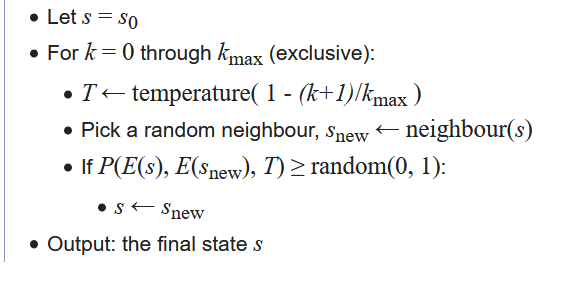
\includegraphics[width=1\linewidth]{screens/pseudocode}
	\caption{Pseudo-kod głównej części algorytmu simulated annealing}
	\label{fig:pseudocode}
\end{figure}


Algorytm działa $ k_{max} $ razy w pętli for,
w pierwszym kroku każdej iteracji jest przypisywana nowa temperatura zwracana z funkcji annealling temp


\paragraph{wersja druga}
Drugie podejście charakteryzowało się innym podejściem do zmian temperatury

inne podejście do epoki (iteracji po jednej temperaturze), może mieć kilka prób dla jednej epoki,

zmiana podejścia do sąsiedztwa w kontekście jednej epoki

głowne zalorzenie to zmniejszanie zakresu wyboru/uzaleznienie losowosci od temp


\subsection{algorytm genetyczny}


\subsection{wyniki}





\section{Problemy}
Indeksacja

wybór następnego kandydata na rozwiązanie




\end{document}
